% Article type supporting font formatting
%\documentclass[10pt]{extarticle}
\documentclass[a4,10pt]{article}

% Define .tex file encoding
\usepackage[utf8]{inputenc}

% Norwegian language support
%\usepackage[norsk]{babel}     

% Indent first paragraph in section
\usepackage{indentfirst}

% Allows mathbb in tex file
\usepackage{amsfonts}    
     
% Margin defining package
%\usepackage{geometry}         
%\geometry{a4paper
  %,margin=.75in
%}

% For use of graphics in document
\usepackage{graphicx}         

% Allows multi-line comments in tex file
\usepackage{verbatim}         

% Allows math in tex file 
\usepackage{amsmath}          

% Allows math symbols in tex file
\usepackage{amssymb}          

% Allows use of physics shortcut functions
\usepackage{physics}          

% Verbatim env with LaTeX commands
\usepackage{alltt}            

% Allows \begin{figure}[H]
\usepackage{float}            

% Necessary for defining colours
\usepackage{color}            
\definecolor{linkgreen}{rgb}{0,.5,0}
\definecolor{linkblue}{rgb}{0,0,.5}
\definecolor{linkred}{rgb}{.5,0,0}
\definecolor{blue}{rgb}{.13,.13,1}
\definecolor{green}{rgb}{0,.5,0}
\definecolor{red}{rgb}{.9,0,0}

% Hyperlinks in document
\usepackage{hyperref}  
\hypersetup{
  colorlinks=true,     % True for colored links
  linktoc=all,         % True for table of contents links
  linkcolor=linkblue,  % Colour for links
  urlcolor=linkgreen,  % Colour for URLs
  citecolor=linkred    % Colour for citations
}

% Listing package for code examples
\usepackage{listings}         
\lstset{
  language=C++,                % Set language to C++
  showspaces=false,            % Don't show space chars
  showtabs=false,              % Don't show tab chars
  breaklines=true,             % Break long lines of code
  showstringspaces=false,      % Don't show spaces in strings
  breakatwhitespace=true,      % Break at white space only
  commentstyle=\color{green},  % Set colour for comments
  keywordstyle=\color{blue},   % Set colours for keywords
  stringstyle=\color{red},     % Set colour for strings
  basicstyle=\ttfamily,        % Set basic style
  tabsize=2                    % Set tabsize
}

% Referencing, last for compatibility reasons
\usepackage[noabbrev]{cleveref}

% Command to set two lines under text
\newcommand{\uunderline}[1]{\underline{\underline{#1}}}

% Command to use integral with limits
\newcommand{\Int}{\int\limits}    

% Command to use double integral with limits
\newcommand{\IInt}{\iint\limits}  

% Command to use triple integral with limits
\newcommand{\IIInt}{\iiint\limits}

% Command removes section numbering
\newcommand{\mysection}[2]{   
\setcounter{section}{#1}
\section*{#2}
\addcontentsline{toc}{section}{#2}
}

% Command removes subsection numbering
\newcommand{\mysubsection}[2]{  
\setcounter{subsection}{#1}
\subsection*{#2}
\addcontentsline{toc}{subsection}{#2}
}

% Command removes subsubsection numbering
\newcommand{\mysubsubsection}[2]{ 
\setcounter{subsubsection}{#1}
\subsubsection*{#2}
\addcontentsline{toc}{subsubsection}{#2}
}

% Makes matrices look square-ish
\renewcommand*{\arraystretch}{1.5}

%%%%%%%%%%%%%%%%%%%%%%%%%%%%%%%%%%%%%%%
%%      Title, Author, and Date      %%
%%%%%%%%%%%%%%%%%%%%%%%%%%%%%%%%%%%%%%%
\title{Finite Element Method Programming Report}
\author{Daniel Aaron Salwerowicz}
\date{\today}

%%%%%%%%%%%%%%%%%%%%%%%%%%%%%%%%%%%%%%%
%%           Start document          %%
%%%%%%%%%%%%%%%%%%%%%%%%%%%%%%%%%%%%%%%
\begin{document}
  
%%%%%%%%%%%%%%%%%%%%%%%%%%%%%%%%%%%%%%%
%%   Create the main title section   %%
%%%%%%%%%%%%%%%%%%%%%%%%%%%%%%%%%%%%%%%
\maketitle

%%%%%%%%%%%%%%%%%%%%%%%%%%%%%%%%%%%%%%%
%%      Abstract for the report      %%
%%%%%%%%%%%%%%%%%%%%%%%%%%%%%%%%%%%%%%%
\begin{abstract}
  Purpose of this report is to present my work on developing a C++ based solver for Partial Differential Equation (PDE) in $\mathbb{R}^2$ which is based on Final Element Method (FEM). 
\end{abstract}

%%%%%%%%%%%%%%%%%%%%%%%%%%%%%%%%%%%%%%%
%%         ToC for the report        %%
%%%%%%%%%%%%%%%%%%%%%%%%%%%%%%%%%%%%%%%
%\tableofcontents
%\pagebreak

%%%%%%%%%%%%%%%%%%%%%%%%%%%%%%%%%%%%%%
%%  The main content of the report  %%
%%%%%%%%%%%%%%%%%%%%%%%%%%%%%%%%%%%%%%
\section{Introduction}
In this project I have utilized a geometric modeling library developed by Simulations R\&D group at UiT called GMlib. In addition to that I have used Qt, and C++. These tools were used to create a physical simulation of a circular membrane in $\mathbb{R}^2$ affected by a constant, external force. I achieved it by numerically solving Poisson equation describing distortion of the aforementioned object. To simplify the problem I have assumed that the force is applied uniformly and normally to the membrane, I have also disregarded the material properties and time.

After simplifying the original PDE to a weak expression I have implemented methods to discretize the continuous surface using "finite elements", calculate stiffness matrix and load vector, solve the equation for a given force, and show the results in form of an animation.

\section{Methods}
Methods used to solve this problem included:
\begin{enumerate}
  \item Triangulating membrane and defining basis functions.
  \item Calculating stiffness matrix $A$ and load vector $b$.
  \item Solving matrix equation:
  \begin{equation} \label{MatrixEquation}
  x=A^{-1}b
  \end{equation}
  \item Updating position for internal nodes in the triangulated membrane.   
\end{enumerate}

\subsection{Tools used}
\subsubsection{GMlib}
GMlib gave me several useful classes and methods that I've based my solution on. \verb|TriangleFacets| class was used as a basis for \verb|FEMObject| class and \verb|Vertex| class that was used in creating \verb|Node| class. Other classes that were used in this solution inculde \verb|Edge| and \verb|Triangle| as well as \verb|triangulateDelaunay| method. This library came along with a Qt wrapper project called \verb|QmlDemo| that was used to visualize the solution using the Qt 3D modeling engine.

\subsubsection{FEMObject}
This class extends \verb|TriangleFacets| class, which in turn extends \verb|ArrayLX| class. I've used this class to create mesh of vertices used to triangulate the membrane, calculate stiffness matrix and load vector, solving the matrix \cref{MatrixEquation}, and animating the membrane.

\subsubsection{Node}
This class extends \verb|Vertex| class and implements some useful methods that \verb|FEMObject| uses in calculation of $A$ and $b$.

\subsection{Membrane triangulation}
To triangulate membrane in $\mathbb{R}^2$ I've used Delaunay algorithm implementation found in \verb|TriangleFacets| since it's optimal for this case. One of the advantages of Delaunay triangulation is that it maximizes the minimal angle in all of the triangles. Delaunay algorithm requires a mesh of nodes to create triangles, therefore I have defined two types of mesh generation algorithms in \verb|FEMObject|: regular and random. This triangulation will be used to create basis functions where overlapping functions will give me values for the stiffness matrix and load vector.

\subsubsection{Regular mesh generation}

Input values for the \verb|regularTriangulation| method are: \textbf{r} Radius of the membrane. \textbf{n} Number of nodes in the first row of mesh. \textbf{m} Number of rows in mesh.

Distance between every row in mesh is equal to $x = r/m$. Points are added iteratively, staring from node in origin and then moving outwards row by row.
First node in row has coordinates $(x, 0)$. To compute the rotation angle I used the formula $\alpha = i 2\pi / n, \quad i = 0,...,k-1$. $k$ represents number of nodes in a given row, $k = j \cdot n \quad j=1,2,...,m$. To complete each row I add $k$ points with coordinates $R \binom{x}{0}$, where $R$ is the rotation matrix.

In order to represent the rotation angle I have used \verb|Angle| class found in GMLib. While rotation matrix $R$ is represented by \verb|SqMatrix| which when multiplied automatically works as a rotation matrix. %This is how I've solved this problem in code.
\begin{comment}
\begin{lstlisting}
for (int j = 1; j <= m; ++j) {
for (int i = 0; i < n * j; ++i) {
Angle alpha = i * (M_2PI / (n * j));
auto R = SqMatrix(alpha);
auto pos = R * Point(x * j, 0);
insertAlways(Vertex(pos[0], pos[1]));
}
}
\end{lstlisting}
\end{comment}

\subsubsection{Random mesh generation}
Input value for \verb|randomTriangulation| method is \textbf{e\_nodes} that represents number of nodes on the boundary. Starting from a regular mesh I have made an algorithm that randomly swaps internal nodes and then deletes 75\% of nodes from the array. Resulting mesh makes it much easier to calculate the displacement of membrane, whilst preserving smoothness of the object that I get from regular mesh.

To perform swapping I used \verb|uniform_int_distribution| defined in std. Then I calculate two values to limit how many times nodes will be swapped and how many nodes will be removed. It's worth noting that I use \verb|removeBack| method, since it's most efficient removal method in \verb|ArrayLX|. This method works best with meshes that have a lot of elements to begin with, meshes with relatively few (under 100) nodes end up looking too rough. However I don't see is as a problem, since in normal use membrane is triangulated by a lot of triangles.
\begin{comment}
\begin{lstlisting}
auto swap_lim = size() * 3;
auto delete_lim = floor((size() - e_nodes) * 0.75);

for (int i = 0; i < swap_lim; ++i)
swap(dis(gen), dis(gen));

for (int i = 0; i < deleteLimit; ++i)
removeBack();
\end{lstlisting}
\end{comment}

\begin{figure}[H]
  \centering
  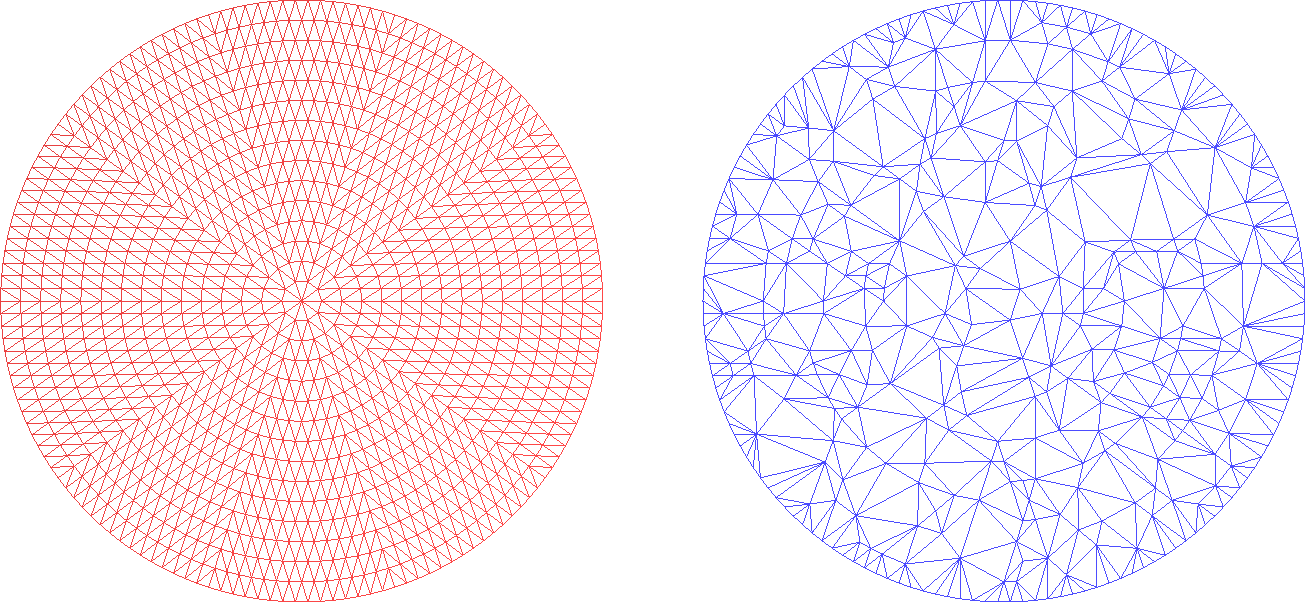
\includegraphics[width=.75\textwidth]{Triangulation}
  \caption{Triangulations made using regular and random meshes}\label{Meshes}
\end{figure}

\subsection{Solving equation}

Defining circular domain $\Omega \in \mathbb{R}^2$ with its boundary  $\partial \Omega$ and applying force $f$ on the domain, Poisson's equation describing it takes the following form.

Find $u$, which is the deformation level of circular membrane, such that
\begin{equation} \label{StrongPoisson}
\left\{
\begin{array}{rll} 
\Delta u = f \text{, in } \Omega, \\
u = 0, \text{ on } \partial \Omega.
\end{array} \right.
\end{equation}
where $\Delta = \pdv[2]{}{x} + \pdv[2]{}{y}$ is the Laplace operator.

Using well defined theory for transforming strong formulation of PDE to weak formulation I got following equation:
\begin{equation} \label{WeakPoisson}
\Int_{\Omega} \Delta v \cdot \Delta u = \Int_{\Omega}f(s) \cdot v \; ds
\end{equation}

Assuming that $\Omega$ is partitioned by $N$ nodes where only internal nodes are taken into consideration I can rewrite \cref{WeakPoisson} as:
\begin{equation} \label{MatrixFormulation}
Ax=b
\end{equation}
For brevity I have omitted showing all necessary calculations to arrive at this result. They can be found in lecture notes provided on Canvas. \cite{Kravetc:2018}

\subsection{Calculation of stiffness matrix}
\subsubsection{Non-diagonal elements}
Values for elements $a_{ij}$ in stiffness matrix A are zero if there's no edge between them. If there exists an edge $ij$ then the value of $a_{ij}$ can be calculated using two triangles that have edge $ij$.
\begin{equation} 
\begin{aligned}\label{NonDiagAElement}
a_{ij} &= \left( \frac{-1}{|d|^2} + \frac{a_1 \cdot d}{|d \times a_1|} \left(1 - \frac{a_1 \cdot d}{|d \times a_1|}\right)\right)\frac{|a_1 \times d|}{2}\\ &+ \left( \frac{-1}{|d|^2} + \frac{a_2 \cdot d}{|d \times a_2|} \left(1 - \frac{a_2 \cdot d}{|d \times a_2|}\right)\right)\frac{|a_2 \times d|}{2}
\end{aligned} 
\end{equation}
Where $d$ is the vector between $i$ and $j$, while $a_1$ and $a_2$ are vectors that go from $i$ to vertices in the two triangles that lie on the intersection of two nodes and have $ij$ as an edge.

To find vectors $\overrightarrow{a_1}$ and $\overrightarrow{a_2}$ in code I have set up my program to find points $P_2$ and $P_3$, then subtract $P_0$ from them to get vectors. I get triangle vertices by calling \verb|triangle->getVertices()| method which returns array of \verb|Vertex| objects. Then I go through vertex array and find one that doesn't have $P_0$ or $P_1$ as their parameter. The $\overrightarrow{d}$ is found by calling \verb|edge->getVector()| method.

\subsubsection{Diagonal elements}
Values for diagonal elements are simply expressed as
\begin{equation} \label{DiagAElement}
a_{ii} = \sum_{k=1}^{\ell} T_k=\frac{d_3 \cdot d_3}{2 |d_1 \times d_2|}
\end{equation}
Where $\ell$ is the number of triangles that have corner in $i$, and $d_1$, $d_2$ and $d_3$ are vectors that form edges of triangle $T_k$.

To find these three vectors I get array of vertices from \verb|triangle->getVertices()| and then order them so that first object in array is $P_0$, second is $P_1$ and last one $P_2$.

\subsection{Calculation of load vector}
The load vector $b$ is assembled by following formula:
\begin{equation} \label{BElements}
b_i = \Int_{K}fv_i \; ds = f \frac{1}{3} \sum_{k = 1}^{\ell}S_{T_k}
\end{equation}
The function $f$ is the specified load function. An integral of the basis function is equal to the volume of a pyramid based on the node with height equal to 1. An area of the base is equal to the sum of triangle areas $S_{T_k}, \quad k = 1,...,\ell$. Areas of triangle are found using \verb|triangle->getArea()| method.

\begin{figure}[H]
  \centering
  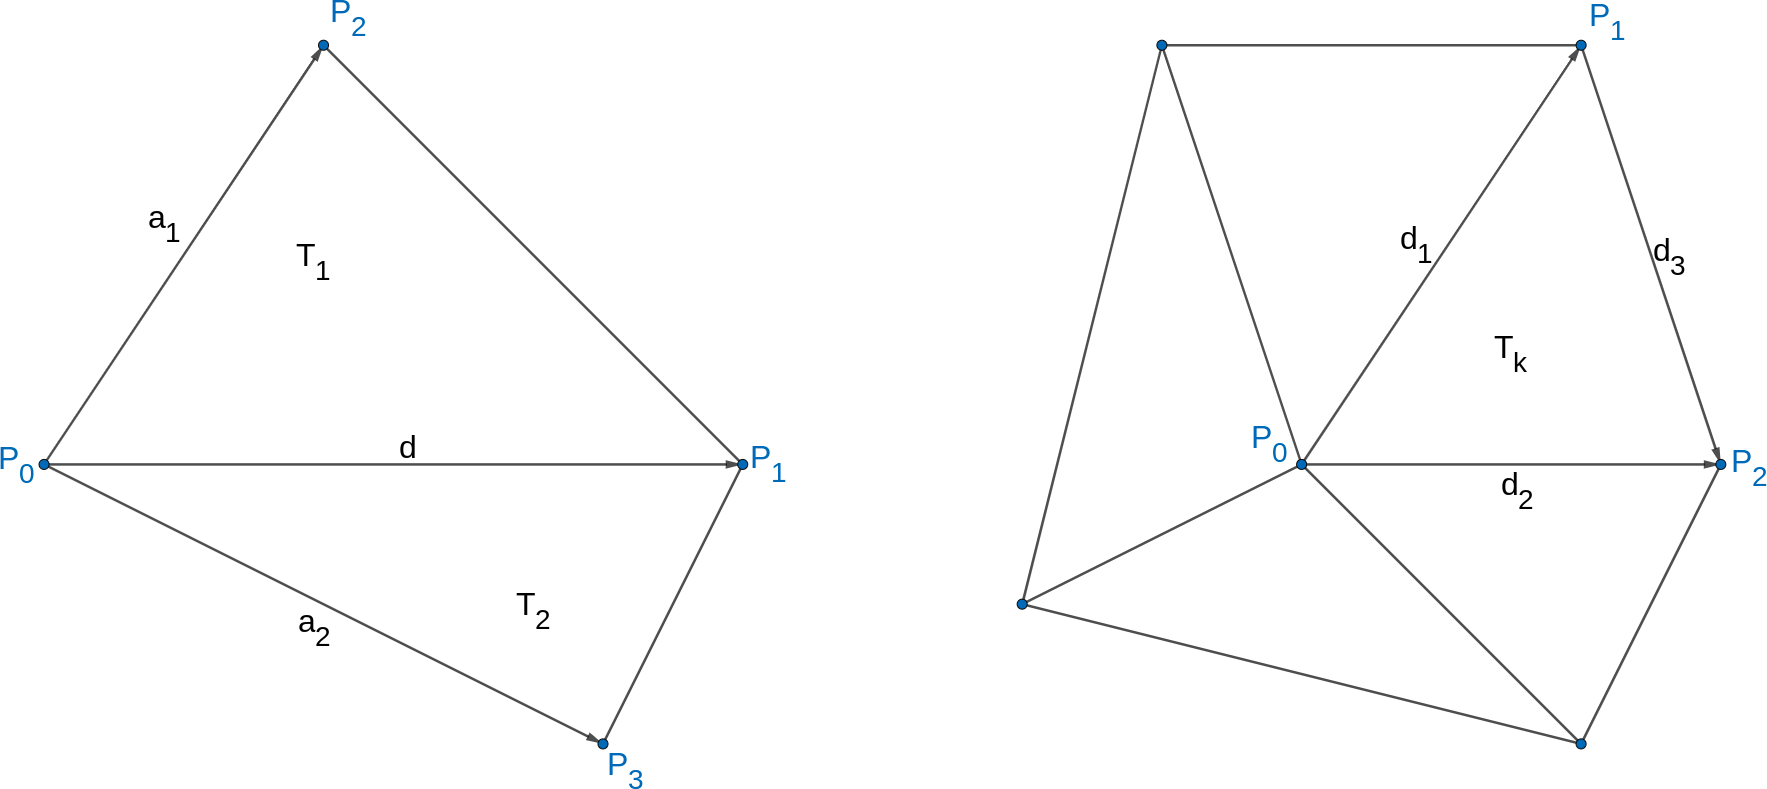
\includegraphics[width=.75\textwidth]{Triangles}
  \caption{Diagrams to better explain how \cref{NonDiagAElement,DiagAElement,BElements} were derived}\label{Triangles}
\end{figure}

\subsection{Animation}
Animating the solution involved adding some helper members and methods to \verb|FEMObject| class and overriding \verb|localSimulate| method. This method simply updates the value of $f$ based on the $dt$, and updates position of internal nodes. $dt$ represents timestep in animation. 

Minor changes to \verb|simulator.h| and \verb|simulator.cpp| files were done to call \verb|replot| on \verb|FEMObject| objects in scene. This is simply a method that goes through vector of scene objects and calls \verb|replot| on them. This method was connected in \verb|application/guiapplication.cpp| so that it is called during simulation.

\section{Results}
Using the aforementioned methods I have been able to successfully implement a program that is able to simulate distortion of a circular membrane. Program can be programmed to use regular and random triangulation, change maximum force, and speed of animation.

There exists a bug in animation itself. When it is run at sufficiently high speed, speed factor set to be under 0.2, then the membrane might stop at one of the peaks and stop updating its position. I was unable to resolve this problem as I needed to focus on other projects and exams.

Video showing the animation can be found in the project directory or by following this link: \url{https://youtu.be/wwwnGKdEI7A} 

\begin{figure}[H]
  \centering
  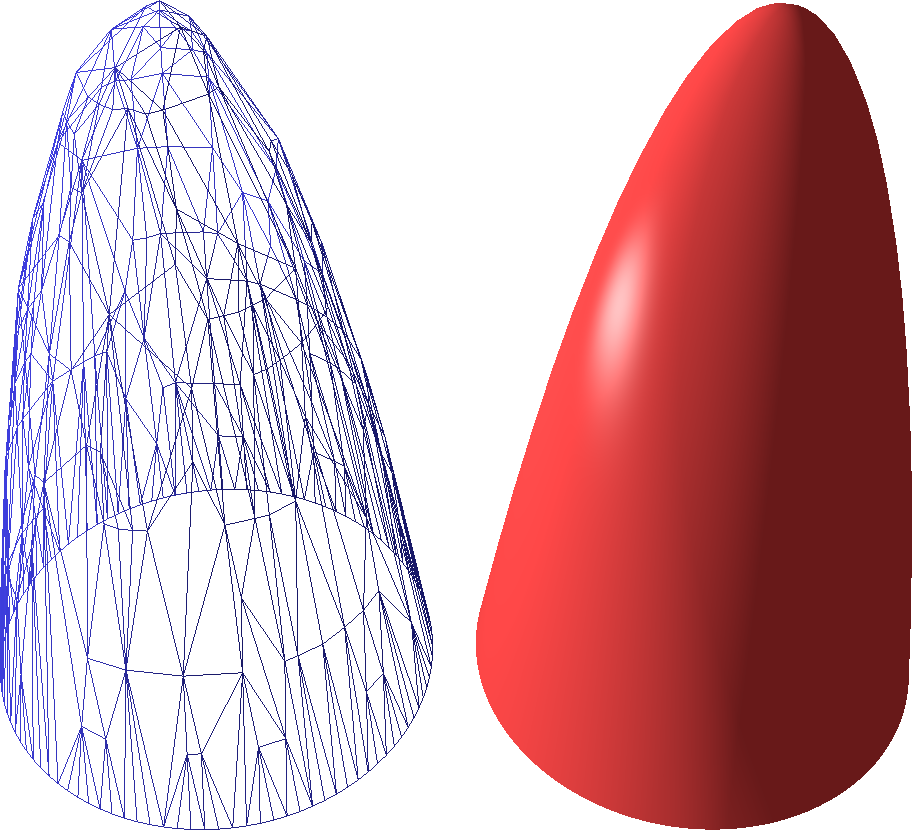
\includegraphics[width=.65\textwidth]{Distortion}
  \caption{Distortion of membrane calculated using my program}\label{Distortion}
\end{figure}

\section{Analysis \& Discussion}
After consultation with Tatiana Kravtec and Arne Laks\aa{} I am sure that my program functions correctly and finds the proper distortion for a given force. Furthermore the animation runs very smoothly provided I use random triangulation instead of regular one, as the number of necessary calculations for regular triangulation slows down the program too much. 

Even though I haven't run benchmarks on my code, it's clear that the program runs fast. The big bottleneck is visualization of results in 3D. This claim based on a test run on a regularly triangulated membrane with 15 nodes in first row and 20 rows. Calculation itself took around 5 seconds on my computer while it took 15 minutes to show the result on my computer. 

Using an iterative method for inverting and multiplying matrices would cut down on calculation time greatly. All of the professional FEM products implement that, which cuts down on calculation time greatly. Seeing how a lot of element in $A$ are zero using a textbook version of matrix inversion takes too much time on a huge matrix. In my opinion this is the main bottleneck in my program. 

Further development can be done. It would be very good to implement a way to change triangulation method on the fly or change value for max force or animation speed in the GUI, instead of hard-coding these values in program. I should also fix animation error that was mentioned in the results section. Another improvement would be to have a function that deletes nodes that are very close to each other to cut down on calculation time. Another function that if there are too few nodes in an area and fixing that would be a good choice too.

\section{Bibliography}
\begingroup
  \def\section*#1{}
  \bibliographystyle{plain}
  \bibliography{Bibliography}
\endgroup

\end{document} 